
% Take from PyAudioAnalysis
% short-term, mid-term features

% \chapter{Algorithms}
% \section{Time Analysis}
% \subsection{Convolution}
% A general use of the convolution operation
% is to evaluate the outputs of linear
% time-invariant systems.
% Taking the impulse response of a system, and
% applying the convolution with
% a given input, gives the system's output
% for that specific input.

% For continuous time dependent arguments,
% \(x\) as the input variable, and \(h\) as the
% system's impulse response, the convolution is given by:

% \begin{equation}
%     (x * h)(t) \triangleq \int^{\infty}_{-\infty} x(t)h(t-\tau) d\tau
% \end{equation}

% Due to the commutativity property of the convolution
% operation, the shifting over one of the arguments
% is interchangeable, thus one can write
% the same equation as:

% \begin{equation}
%     (x * h)(t) \triangleq \int^{\infty}_{-\infty} x(t-\tau)h(t) d\tau
% \end{equation}

% Likewise, working with discrete variables,
% the convolution operation can be written as:
% \begin{align}
%     (x * h)[n] \triangleq & \sum^{\infty}_{m=-\infty} x[m]h[n-m] \\
%     (x * h)[n] \triangleq & \sum^{\infty}_{m=-\infty} x[n-m]h[m]
% \end{align}


% \subsection{Cross-Correlation}
% Cross-correlation is an operation that can measure
% how similar two functions are. By ``shifting''
% one function over the other and measuring the amount
% of correlation at each given point, the output graph
% demonstrates at what ``distance''
% the maximum similarity occurs,
% in correspondence
% to the graph's maximum amplitude.

% \begin{align}
%     (x * h)(t) \triangleq & \int^{\infty}_{-\infty} x^{*}(t)h(t+\tau) d\tau \\
%     (x * h)(t) \triangleq & \int^{\infty}_{-\infty} x^{*}(t-\tau)h(t) d\tau
% \end{align}

% \begin{align}
%     (x * h)[n] \triangleq & \sum^{\infty}_{m=-\infty} x^{*}[m]h[n+m] \\
%     (x * h)[n] \triangleq & \sum^{\infty}_{m=-\infty} x^{*}[n-m]h[m]
% \end{align}

% \subsection{Auto-Correlation}
% In a case where the two input functions
% of the cross-correlation are the same input signals,
% the measure is then called ``auto-correlation''.
% In other words, this measure demonstrates
% at what ``distance'' the delayed version of the signal
% most matches the original version of it.

% This kind of measure is very useful in audio
% applications where multi-microphones are spread
% with varying distance from each other and from the
% source. Looking for the maxima point of the
% auto-correlation between the signal received by
% the microphones, one can deduce the lag time
% that best characterizes the microphones' formation.

% Several enhancement and manipulation techniques
% are then become available when the lagging
% time is known.
% For example the delay and sum algorithm beamforming
% algorithm for constructive summation of the different
% channels that translates
% to better SNR (signal-to-noise ratio).

% \subsubsection{Covariance Matrices}
% \begin{equation}
%     \mathbf{R}_{XY} \triangleq \mathbf{E}[XY^{tr}]
% \end{equation}

% \begin{align}
%     \mathbf{R}_{XX} & \triangleq \mathbf{E}[XX^{tr}] \\
%                     & = \frac{1}{T} \sum^{T-1}_{t=0}
%     {X}(t;j\omega){X}^{\mathbf{H}}(t;j\omega)
% \end{align}

% Where the \(\mathbb{H}\) operator
% is the \emph{Hermitian function} which stands for
% the complex conjugate.

% % ESPNet \& Mirco Document
% \subsection{Sinc-Conv}

% % \begin{figure}[ht]
% %     \centering
% %     \includegraphics[width=0.99\textwidth]
% %     {./img/Comparison_convolution_correlation.svg}\label{fig:conv_vs_corr_plot}
% %     \caption{Convolution vs. Cross-Correlation vs. Auto-Correlation plot [Wikipedia]}
% % \end{figure}



% \section{Frequency Analysis}
% \subsection{DTFT}
% \begin{equation}
%     X_{2\pi}(\omega) = \sum_{n=-\infty}^{\infty} x[n] \,e^{-i \omega n}
% \end{equation}


% \subsection{IDTFT}
% \begin{equation}
%     x[n] = \frac{1}{2 \pi}\int_{2\pi} X_{2\pi}(\omega)\cdot e^{i \omega n} d\omega
% \end{equation}

% \subsection{DFT}
% \begin{equation}
%     \label{eq:dft}
%     X_k = \sum_{n=0}^{N-1} x_n \cdot e^{-\frac {i 2\pi}{N}kn}
% \end{equation}

% Taking Euler's identity:
% \begin{equation}
%     e^{ix} = \cos x + j\sin x
% \end{equation}

% Substituting the exponent power in Equation\;\ref{eq:dft} with the Euler identity
% gives:
% \begin{equation}
%     X_k = \sum_{n=0}^{N-1} x_n \cdot \left[\cos\left(\frac{2 \pi}{N}kn\right)
%         - i \cdot \sin\left(\frac{2 \pi}{N}kn\right)\right]
% \end{equation}


% \subsection{IDFT}
% \begin{equation}
%     x[n] = \frac{1}{N} \sum_{k=0}^{N-1} X_k\cdot e^{i \frac{2 \pi}{N} k n}
% \end{equation}


% \subsection{FFT --- Fast Fourier Transform}

% \subsection{Discrete Cosine Transform (DCT)}

% \begin{equation}
%     y[n] = \sum^{}_{}
% \end{equation}

% \section{Time-Frequency Analysis}
% \subsection{STFT - Short Time Fourier Transfer}

% \subsection{Spectrogram}

% \section{Windows}
% \subsection{Overview}


% \subsection{Rect (boxcar)}
% \subsection{Triangle}
% \subsection{Bartlett}
% \subsection{Hamming}
% \subsection{Hann}
% \begin{align}
%     w[n] = 0.5 - 0.5\cos\left( \frac{ 2\pi n }{ M - 1 } \right) & \qquad 0 \leq n \leq M-1
% \end{align}


% % \subsection{Kaiser}
% % \subsection{Analog Filters}

% \subsection{Overlap + Add Reconstruction}
% % \subsection{Wavelets}

% \section{Speech-Enhancement}
% See table
% \begin{figure}[ht]
%     \centering
%     \includegraphics[width=0.99\textwidth]
%     {./img/spc_enhance_tbl}\label{fig:asr_blocks_diagram}
%     \caption{General E2E ASR System Blocks Diagram}
% \end{figure}



% DCT + MFCC Connection
% DST - Discrete Sine Transforms
% Hilbert Transform
% Analytical Signal
% Wavelates
% Convolution / Correlation
% Parseval's Theorm
% PSD
% Median Filter
% ORder Filter
% Wiener Filter
% Hermitian FFTs





\chapter{Features}\label{ch:features}
\section{Introduction}
In data analysis craftsmanship,
it is important to characterize the data so that
variations are noticeable and more easily discernible
during the analysis process.
To that end, the input data being analyzed is reorganized
according to selected features on which
conclusions and distinctive deductions can be made.
Similarly, in a supervised learning 
procedure, data reorganization is needed
in order to make classification decisions accurately. 

An intelligent choice of the learnable features 
\cite{7845025} 
can drastically change a given model's outcomes quality.
In supervised learning, the 
feature selection and extraction process withal,
are preparatory steps to the learning or classification
stages coming next.
As a rule of thumb, the more features, the better accuracy
a learning model can yield theoretically\cite{lessIsMore}.
That saying holds true to a great degree
as long as the amount of sudden fluctuations do not characterize the data.
In a case of heavy fluctuating data,
or alternatively, in the case of a 
massive number of features, 
that some of which have minor contributions 
to the classification part of the output,
an increase in the number of features may become deteriorative.
In terms of performance, 
enlarging the number of features leads to a bigger model, 
an increased number of learnable parameters, 
longer training times, 
and unnecessary extension of processing times.
Also, a possible reduction in the accuracy is 
expected due to 
False-Negative (FN) or False-Positive (FP) 
misdetections resulting from the wrong 
classification of signals as noise and 
vice versa caused by additional redundant features.

For speech signals, a wide variety of 
meaningful feature sets exist. 
More or less useful, different speech features 
may better fit certain use-cases or fulfill 
a particular unerring task. 
Features for speech (including audio) 
are mainly from the following domains:
\begin{enumerate}
    \item Spectral Features
    \item Cepstral Features
    \item Time domain Features
    \item Spatial Features
\end{enumerate}

Speech features are selected 
to give the maximal accuracy in detecting utterances.
That means a precise characterization of a 
word, utterance, or the pronunciation of 
a single character, making them distinguishable
from other input streams. 

\section{Spectral Features}
\subsection{FB -- FilterBanks}
Utilizing FilterBanks is a very common technique
for spectral mapping of speech signals.
By dividing the audio spectrum into multiple 
sub-domains with a defined level of overlap, 
the spectrum is 
``framed'' according to frequency. 
Thus, by a set of band-pass filters,
each frame contains the confined 
information of the speech signal 
that corresponds to the filter's specific 
range of frequencies.

The resolution can then be set as a function of
the number of filters and the overall processed audio bandwidth.
Increasing the number of filters, assuming the 
audio bandwidth and the overlap ratio are constant, means
narrower allocated bandwidths for each individual filter
or in other better spectral resolution.

Filterbanks by themselves are not the desired speech feature,
but only the mean for feature extraction. 
The most common feature extracted by a Filterbank set
is the total sum of energy bounded by the filter's frequency response.
A set of filters is computed per 
frequency bin and remains the same for 
the entire signal length over time.
Thus, the total sum of energy computed for 
each filter characterizes the 
speech over a finite defined duration of time.

The human hearing system is less sensitive to high frequencies
than lower band frequencies, as described in Chapter\;\ref{ch:scaling_methods}.
Therefore, in an attempt to emulate the same natural behavior and
resemble the hearing ``filters'' as much as possible, 
the Filterbank set of filters is set with center frequencies
according to the different scaling 
methods described in Chapter\;\ref{ch:scaling_methods}.
In that way, narrow-band filters are assigned to 
lower frequency ranges. 
Similarly, wide-band filters are for 
the higher hearable frequency ranges.

\subsubsection{Mel FB}
One way of mapping the audio spectrum is according to the Mel
scale. This scaling method is described in Chapter\;\ref{ch:scaling_methods}.
First, the center frequencies and the bandwidths are received by the transformation
between Hertz to Mels. Then a set of Bartlett
filters with those center frequencies are generated
with an overlap of 50\% between adjacent filters. 


The amplitude of the filters is bounded to ``\(1\)''
to maintain Nonzero Overlap Add (NOLA) compatibility.
An example of a Mel Filterbank constructed by Bartlett filters
is shown in Figure~\ref{fig:sb_mel_fb}.
\begin{figure}[H]
    \centering
    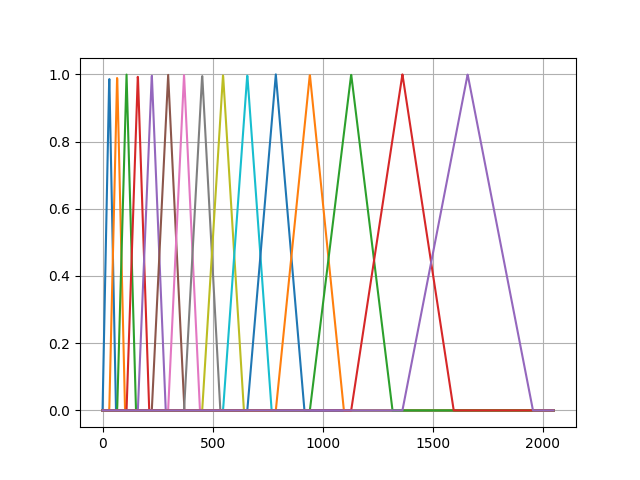
\includegraphics[width=0.75\linewidth]{Features/images/sb_mel_fb}
    \caption{Mel FB}\label{fig:sb_mel_fb}
\end{figure}

\subsubsection{Bark FB}
The Bark Filterbank is very similar to the Mel Filterbank
except that it follows the Bark scale 
instead of the Mel Scale.

Different filter shapes are available but, 
triangular filter shapes are the most common,
as described in \cite{barkfilt}.

An example of the Bark Filterbank constructed by Bartlett filters
is shown in Figure~\ref{fig:mat_bark_fb}.
\begin{figure}[H]
    \centering
    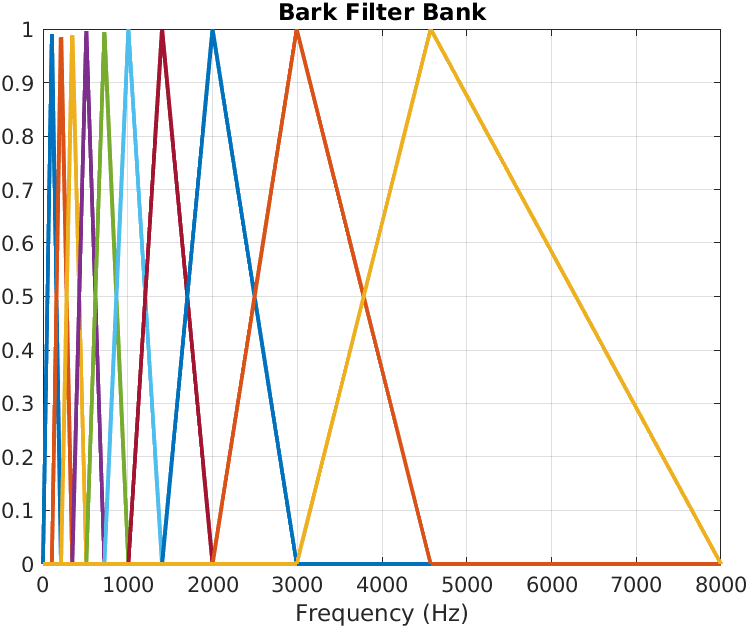
\includegraphics[width=0.75\linewidth]{Features/images/mat_bark_fb}
    \caption{Bark FB}\label{fig:mat_bark_fb}
\end{figure}

\subsubsection{Gammatone FB}
The Gammatone filter, as described in \cite{gammatonefilt},
has a response function as follows:
\begin{equation}
    g(t) = \alpha t^{n-1}e^{-2\pi bt}\cos \left( 2\pi f_{c} t + \phi\right)
\end{equation}

Where \(\alpha\) denotes the amplitude factor,
\(n\) is the filter order,
\(f_{c}\) is the center frequency,
\(\phi\) is the phase factor,
and \(b\) is the bandwidth parameter
computed according 
to the ERB scale mapping of \(1.019\cdot ERB \left( f_{c} \right)\).

An example of a Gammatone Filterbank
is shown in Figure~\ref{fig:sb_fb_gauss}.
\begin{figure}[H]
    \centering
    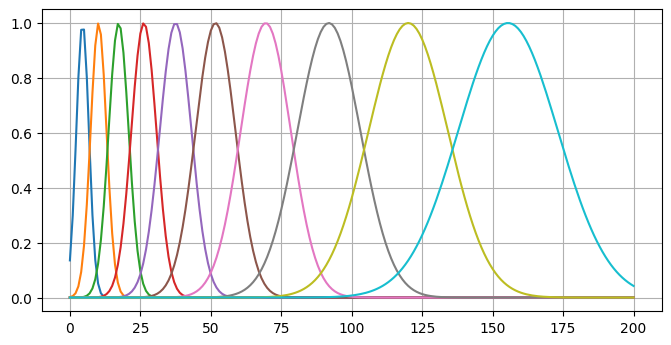
\includegraphics[width=0.75\linewidth]{Features/images/sb_fb_gauss}
    \caption{Gammatone FB}\label{fig:sb_fb_gauss}
\end{figure}


\section{Cepstral Features}
\subsection{MFCCs -- Mel-Frequency Cepstral Coefficients}

% https://link.springer.com/content/pdf/bbm%3A978-3-319-03116-3/1.pdf
\subsubsection{Pre-emphasis}
Speech signals have a roll-off frequency 
resembling a low-pass behavior\cite{237532}.
Due to that physical nature, higher frequencies 
decay faster than lower speech frequencies.
Compensation for this phenomenon is attainable with a 
pre-emphasis filter that boosts 
the higher\cite{7489370} frequencies responses.


\subsubsection{Framing}
Speech signals vary in time. 
Although the variation over time is relatively slow, 
a speech signal is not a pure stationary process 
but a quasi-stationary. 
Therefore, analysis of speech signals 
is taken on small portions of the 
signal to be less affected by randomness effects.
To that end, a preliminary framing action is applied
to speech signals in the time domain.
Framing means dividing the signal 
into small fragments(frames) with some overlapping in between.
Each time frame is assumed to be stationary,
and thus a measurement can be taken.

The shifting in time between frames is referred
to as the hopping length and is set to contain 
a sufficient amount of temporal
context that characterizes the natural
characteristics of speech.

A very common sampling frequency of audio signals
is \(16KHz\). 
As a result, and in order to work with 
a round number of sampling points, 
the frame lengths 
and the hopping lengths 
are set to \(25ms\), and 
\(6.25ms\) or \(10ms\) for hopping size. 
These values translate to a frame length
equals 400 sampling points, and hopping size
equals 100 or 160 sampling points, respectively.
Another advantage of setting the hopping length
as \(6.25ms\) is that it gives
a complete temporal context of 3 adjacent frames
by definition.

\subsubsection{Windowing}
In order to extract each frame only 
whilst also minimizing the Gibbs effects as much as possible,
a windowing function is applied.
As a result, the information confined 
in a given frame is extracted while the 
window's response function tapers 
the edges to reduce the adjacent frames' effect.

Usually, a Hamming or a Hann window 
is used as the window function due to their 
relatively decent trade-off between edge tapering, 
implementation simplicity, bandwidth, and spectral leakage, 
making them exceptionally suitable for speech signals.

The Hamming and Hann windows are given by
Equations\;\ref{eq:hammwin} and \ref{eq:hannwin}, respectively.
\begin{align}
    \label{eq:hammwin} &W_{_{Hamming}}[n] = 0.54 - 0.46
    \cos\left( \frac{2\pi n}{M-1} \right) &
            0 \leq n \leq M - 1 \\
    \label{eq:hannwin} &W_{_{Hann}}[n] = 0.5 - 0.5
            \cos\left( \frac{2\pi n}{M-1} \right) &
            0 \leq n \leq M - 1
\end{align}

\subsubsection{DFT spectrum}
Each one of the windowed frames is
converted to the frequency domain by applying the 
Discrete Fourier Transform (DFT).
The composition of both windowed framing 
and the DFT is referred to as the 
Short-Time Fourier Transform (STFT).
A technique to visualize the STFT outcome is 
called a spectrogram. The STFT outcome contains 
multiple frequency bins per time frame,
making it a function of \(f, t\).

The DFT is given by:
\begin{align}
    X_{m}(f) = \sum_{n=-\infty}^{\infty} x[n]g[n-mR]e^{-j2\pi fn}
\end{align}

Where \(X_{m}(f)\) denotes the DFT transformation of
a given time frame windows signal,
\(g[\circ]\) denotes the window function of size \(M\),
and \(R\) represents the hopping size.

\begin{figure}[H]
    \centering
    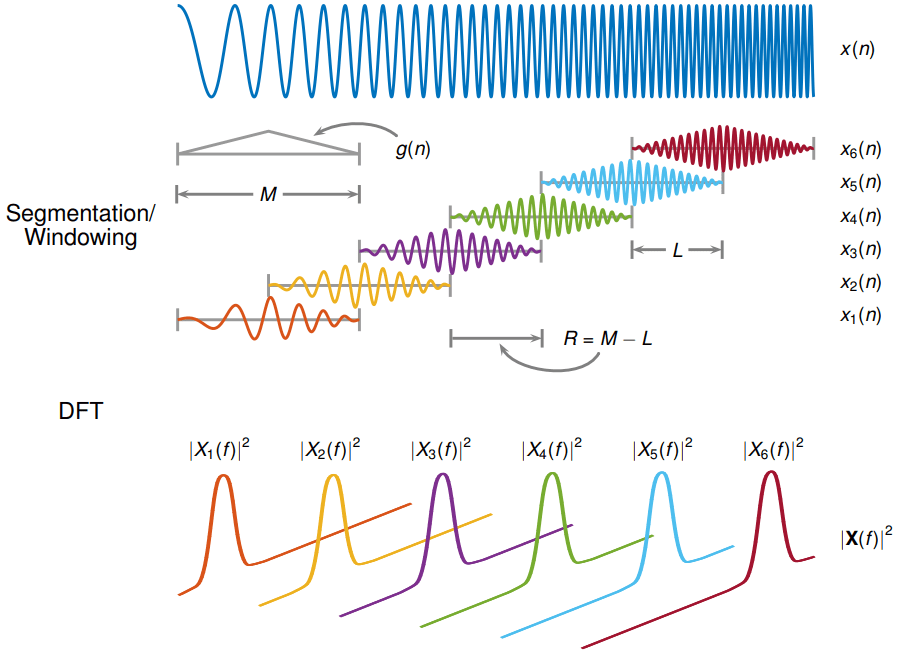
\includegraphics[width=\linewidth]{Features/images/iscola_stft}
    \caption{STFT demonstration diagram}\label{fig:iscola_stft}
    \source{Adapted from Matlab's STFT documentation\cite{matlabStftDoc}}
\end{figure}

\subsubsection{Mel-spectrum}
Once the spectrogram is received, 
the frequencies are rescaled in accordance with the Mel Scale.
A comprehensive description of the Mel Scale 
is detailed in Chapter\;\ref{ch:scaling_methods}.

Next, the cepstral coefficients are extracted from each frequency bin, 
by taking the energies summed of each filter and multiplying it
with the Discrete Cosine Transform (DCT).
\begin{align}\label{eq:mfcc}
    MFCC[n] & = \sqrt{\frac{2}{K}} \sum_{k=1}^{K} \left\{ 
        e[k] \cdot DCT\left( k \right)
     \right\} \nonumber \\
     & = \sqrt{\frac{2}{K}} \sum_{k=1}^{K} \left\{ 
        e[k] \cdot \cos \left( \frac{\pi n}{K} (k+0.5) \right)
     \right\}
\end{align}

It is very common to extract the log-Mel energies
and then have Equation\;\ref{eq:mfcc} written as:
\begin{align}\label{eq:logmfcc}
    MFCC[n] & = \sqrt{\frac{2}{K}} \sum_{k=1}^{K} \left\{ 
        \log \left( e[k] \right) \cdot \cos \left( \frac{\pi n}{K} (k+0.5) \right)
     \right\}
\end{align}

% Take from PyAudioAnalysis
% PyAudioProcessing

\subsection{RFCCs -- Root-Frequency Cepstral Coefficients}
An alternative to the log-Mel 
extraction of the cepstral coefficients
has been suggested in \cite{rmfcc1} and \cite{1415167}.
The motivation to put this proposed 
technique under test is that the root 
function can be less computationally demanding 
than the traditional log function..
\begin{align}
    RFCC[n] & = \sqrt{\frac{2}{N}} \sum_{k=1}^{K} \left\{ 
        \left( e[k] \right)^{\gamma} \cdot \cos \left( \frac{\pi n}{K} (k+0.5) \right)
     \right\}
\end{align}

\subsection{GFCCs -- Gammatone-Frequency Cepstral Coefficients}
GFCCs follow the same basic steps as the MFCCs extraction.
But, instead of translating the frequencies to Mels,
the spectrum is translated to the ERB scale.
ERB scale implies a Gammatone Filterbank as described in Chapter \ref{ch:scaling_methods}.


\subsection{BFCCs -- Bark-Frequency Cepstral Coefficients}
Like the Gammatone-FCCs (GFCCs), the BFCCs follow the Bark scale.

% \subsection{LFCCs --- Linear-Frequency Cepstral Coefficients}
% \subsection{LPC --- Linear Predictive Coefficients}
% \subsection{MSRCC --- Magnitude-based Spectral Root Cepstral Coefficients}
% \subsection{NGCC --- Normalized Gammachirp Cepstral Coefficients}
% \subsection{PNCC --- Mel-Frequency Cepstral Coefficients}
% \subsection{PSRCC --- Mel-Frequency Cepstral Coefficients}
% \subsection{RPLP --- Mel-Frequency Cepstral Coefficients}
% https://spafe.readthedocs.io/en/latest/features/_features.html
% \subsection{articulatory cepstral coefficients}

\section{Time-Domain Features}
\subsection{Dynamic FCC features}
During the framing process, the speech signal 
is divided into small fragments of the speech over time. 
These time unit fragments are called frames.
Each frame spans over a finite time duration.
The extracted cepstral coefficients are computed statically
for a given frame. However, the original speech
is framed in multiple number of frames. 
Therefore, coefficients extractions
have to be dynamic for the entire signal, i.e., all frames.

Additional information about the temporal 
changes between adjacent coefficients can also be extracted
to include the dynamics and transitions within a frame.

\subsubsection{Deltas}
The first derivate of the cepstral coefficients, known as the Deltas (\(\Delta\)),
represents the velocity of the MFCCs' dynamics and 
is a sub-set of the cepstral coefficients.

Deltas (\(\Delta\)) are extracted by:
\begin{equation}\label{eq:deltaderiv}
    \Delta [n] = \frac{ \sum\limits_{i=-T}^{T} k_{i} c_{m}[n+i]}
    {\sum\limits_{i=-T}^{T} |i|}
\end{equation}

Where \(n\) denotes the frame time index, \(k\) marks the 
coefficient weight, \(T\) stands for the number of temporally
adjacent frames used for the calculation, and \(c_{m}\) denotes the
\(m\)th coefficient in the given frame \(n\).

\subsubsection{Delta-Deltas}
Delta-Deltas (\(\Delta\Delta\)) is an extra layer of information
representing the acceleration at which the 
MFCCs' dynamics change within a given time frame.
The extraction of the Delta-Deltas follows the same principale
as the first derivatives. Yet, instead of taking the
cepstral coefficients as the input feature, we replace
\(c_{m}\) in Equation\;\ref{eq:deltaderiv} 
with the first-order derivatives \(\Delta[n]\).

\subsection{Temporal Context}
Temporal context is an attachment of raw unprocessed 
feature data from adjacent
frames together with the currently selected feature. 
Whether spectral, cepstral, or spatial features,
the concatenation of past and future 
features can infer decisions based on a memorized characteristics.
Furthermore, different languages
introduce contextual constraints such as relative positions
of adjectives or nouns to verbs, plurals, affiliations,
possessions, and other lingual principles.

Usually, the number of adjacent past and future frames 
to concatenate is based on the framing and DFT parameters.
It is plain to understand 
one would not want to exaggerate and excessively use
redundant frames that do not have any significant impact
on the accuracy of detection. 
The downside of overly using temporal context frames is potentially having 
orders of magnitude larger amounts of information to process.

% \section{Spatial Features}
% \subsection{VTLN - vocal track length norm}
